\chapter{Design and implementation}

This chapter compares the designs that were made over the course of the project to that of the solution implementation. The designs that are compared are that of the goals, issues and chat. These cover the most important aspects of the platform: collaborative innovation, problem decomposition and communication.

\section{Goals}

\begin{figure}[ht!]
    \centering
    \begin{subfigure}[b]{0.45\textwidth}
        \includegraphics[height=\textwidth, angle=90]{./media/goal_design}
        \caption{The design for viewing a single goal}
        \label{fig:goal-design}
    \end{subfigure}
    ~ %add desired spacing between images, e. g. ~, \quad, \qquad, \hfill etc. 
      %(or a blank line to force the subfigure onto a new line)
    \begin{subfigure}[b]{0.45\textwidth}
        \centering
        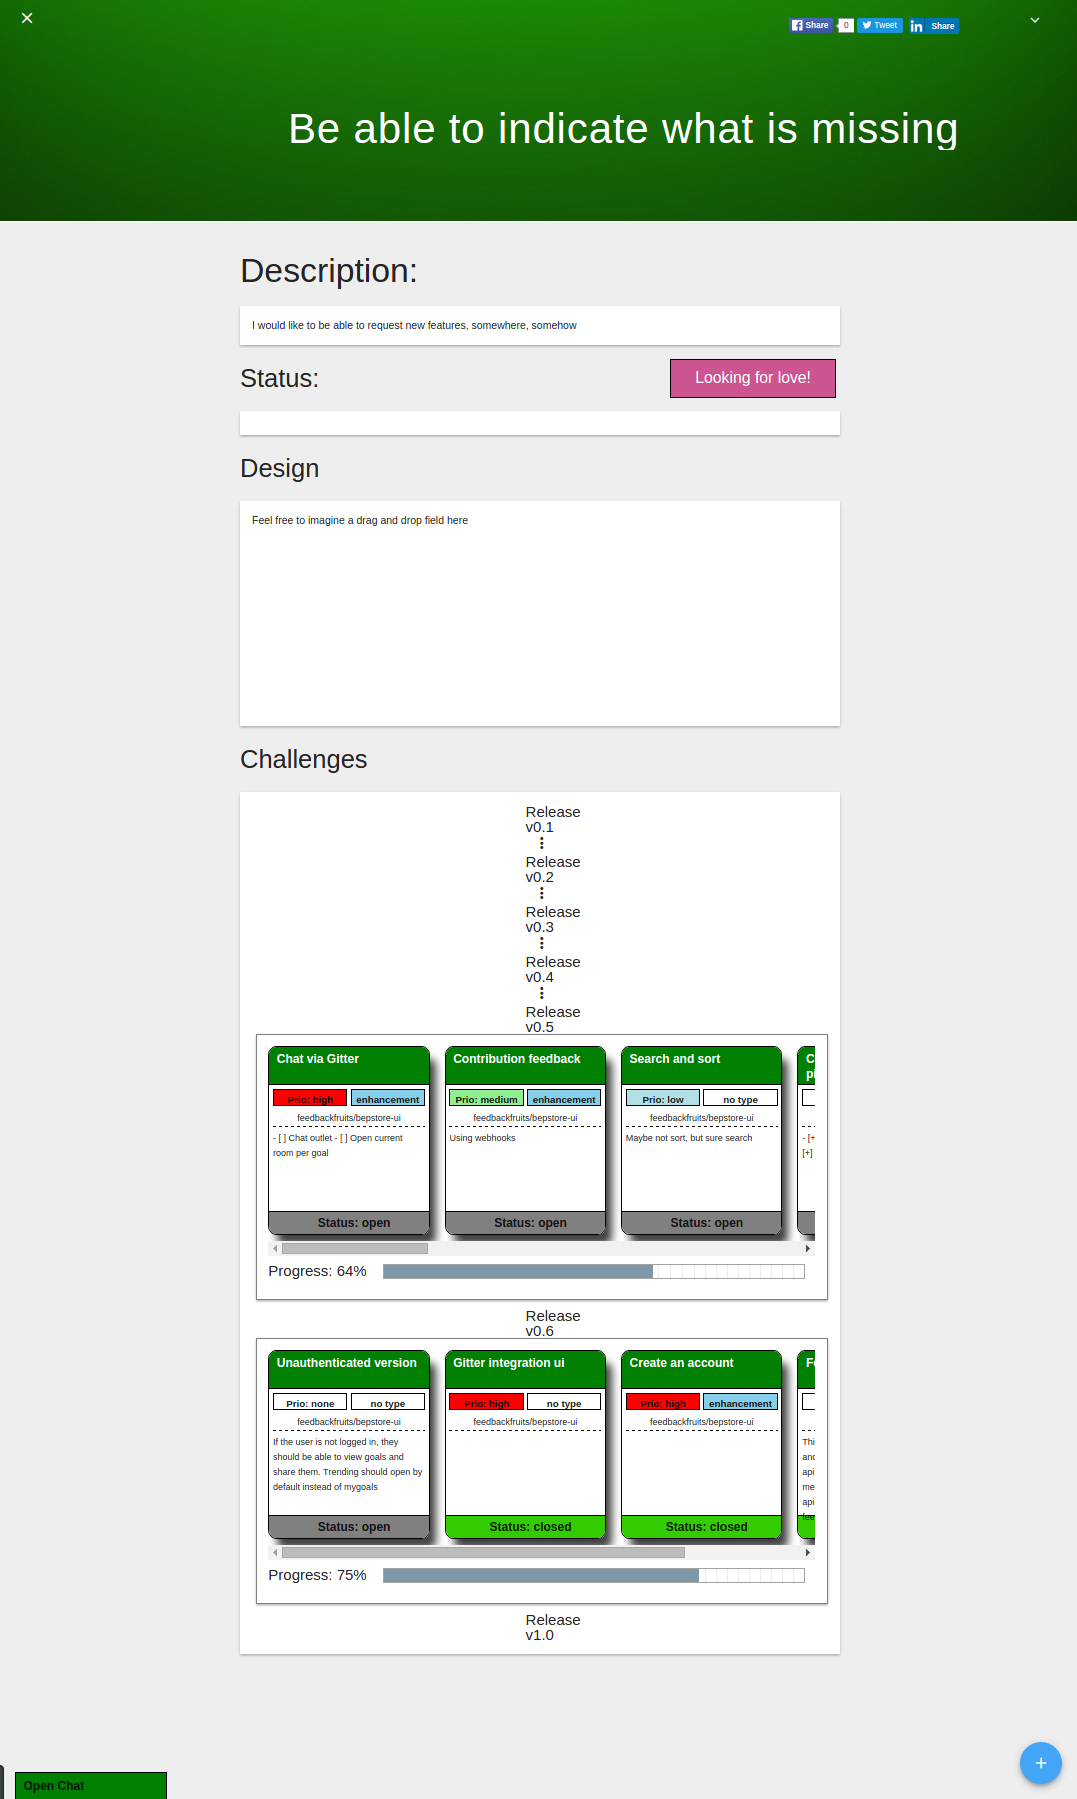
\includegraphics[width=\textwidth, height=0.45\textheight, keepaspectratio]{./media/goal_implementation}
        \caption{The implementation for viewing a single goal}
        \label{fig:goal-implementation}
    \end{subfigure}
\end{figure}
\clearpage
\section{Issues}

\begin{figure}[ht!]
    \centering
    \begin{subfigure}[b]{0.45\textwidth}
        \centering
        \includegraphics[height=0.75\textwidth, angle=90]{./media/issue_design}
        \caption{The design for viewing a single issue}
        \label{fig:issue-design}
    \end{subfigure}
    ~
    \begin{subfigure}[b]{0.45\textwidth}
        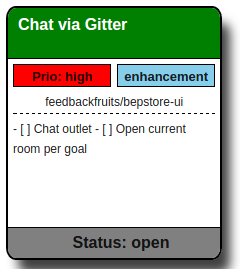
\includegraphics[width=\textwidth]{./media/issue_implementation}
        \caption{The implementation for viewing a single issue}
        \label{fig:issue-implementation}
    \end{subfigure}
\end{figure}

\section{Chat}

\begin{figure}[ht!]
    \centering
    \begin{subfigure}[b]{0.45\textwidth}
        \centering
        \includegraphics[height=0.75\textwidth, angle=90]{./media/chat_design}
        \caption{The design for viewing the chat}
        \label{fig:chat-design}
    \end{subfigure}
    ~
    \begin{subfigure}[b]{0.45\textwidth}
        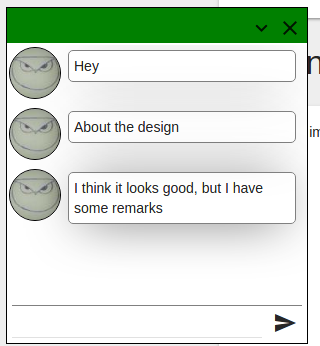
\includegraphics[width=\textwidth]{./media/chat_implementation}
        \caption{The implementation for viewing the chat}
        \label{fig:chat-implementation}
    \end{subfigure}
\end{figure}
